%! TEX program = pdflatex

\documentclass[10pt]{beamer}

\usepackage{graphicx}
\usepackage[utf8x]{inputenc}
% \usepackage{hyperref}
% \usepackage{algorithm}
\usepackage{algorithmic}
% \usepackage{algpseudocode}  
\usepackage{algorithm2e}
% \usepackage[colorlinks, urlcolor=yellow]{hyperref}

\usepackage{cite}


% Reference style
\bibliographystyle{plain}

\usetheme{CambridgeUS}

\hypersetup{colorlinks,linkcolor=yellow,urlcolor=blue}


\title{
    Federated Learning Paper Sharing 
}
\author{
    Lisen Dai
}

\begin{document}
    \maketitle

    \section*{
        FedOpt (Appl. Sci. 2020, 10(8), 2864)
    }
    \begin{frame}
        \frametitle{
            \href{https://www.mdpi.com/2076-3417/10/8/2864}{
            FedOpt: Towards Communication Efficiency and Privacy Preservation in Federated Learning
            }
        }
        \framesubtitle{Sparse Compression Algorithm}
        Goal: reduce the number of communication bits during the models training. \\
        $$
        \Delta\theta = \mathcal{SGD}_n (\theta, D_{mini-batches}) - \theta
        $$
        $\theta$: Deep Neural Network parameters. \\
        $\mathcal{SGD}_n$: refers to the set of gradient updates after n epochs of SGD on DNN (deep neural network) parameters $\theta$ during the sampling of mini-batches from local data \\
        
        Once we have the updates $\Delta \theta$... \\
        
    
    \end{frame}

    \begin{frame}
        \frametitle{
            \href{https://www.mdpi.com/2076-3417/10/8/2864}{
            FedOpt: Towards Communication Efficiency and Privacy Preservation in Federated Learning
            }
        }

        \begin{algorithm}[H]
            % \caption{SCA: Communication Efficiency in FedOpt}
            % \textbf{Initialisation:} \\
            % \textbf{Input:} temporal vector $\Delta \theta$, Sparsity Fraction $q$ \\
            % \textbf{Output:} : sparse temporal $\Delta \theta^*$ \\
      
            % \begin{algorithmic}[1]
            %     % \State{\textbf{Initialisation:}} \newline
            %     % $ num^+ \leftarrow top_{q}(\Delta \theta); num^- \leftarrow top_{q}(- \Delta \theta) $ \newline
            % \end{algorithmic}       
                        
            \KwIn{temporal vector $\Delta \theta$, Sparsity Fraction $q$}
            \KwOut{sparse temporal $\Delta \theta^*$}
            \caption{SCA: Communication Efficiency in FedOpt}
            \label{alg1}
            \textbf{Initialization}\;
            $ num^+ \leftarrow top_{q}(\Delta \theta); num^- \leftarrow top_{q}(- \Delta \theta) $ \\
            $ \Psi^+ \leftarrow mean(num^+); \Psi^- \leftarrow mean(num^-) $ \\
            \If{ $ \Psi^+ \geq \Psi^- $ }{
                \textbf{return} $ (\Delta \theta^* \leftarrow \Psi^+(\theta \geq \min(num^+))) $\;
            }
            \Else{
                \textbf{return} $ (- \Delta \theta^* \leftarrow \Psi^-(\theta \geq \min(-num^-))) $\;
            }
        \end{algorithm}
    
    \end{frame}

    \begin{frame}
        \frametitle{
            \href{https://www.mdpi.com/2076-3417/10/8/2864}{
            FedOpt: Towards Communication Efficiency and
            Privacy Preservation in Federated Learning
            }
        }
        
        \textit{\textbf{“We utilise the additively homomorphic encryption in FedOpt in order to achieve efficiency
        throughout the learning process.”}}

        \begin{figure}[H]
            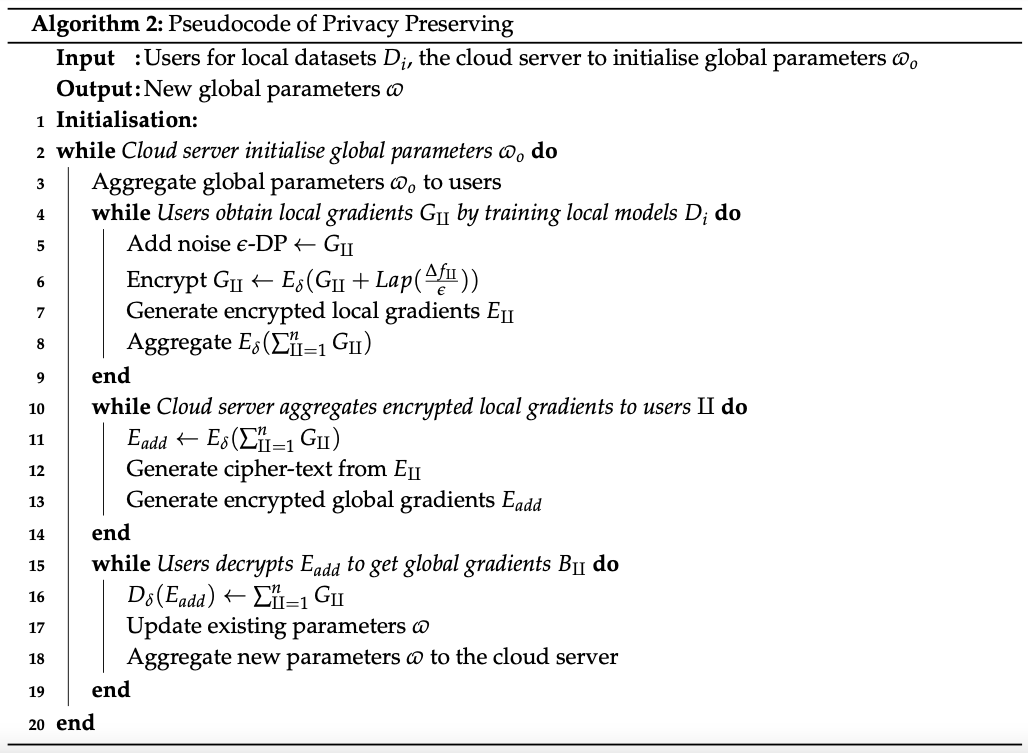
\includegraphics[width=0.8\textwidth]{src/img/Algorithm2.png}
        \end{figure}

    
    \end{frame}


    \begin{frame}
        \frametitle{
            \href{https://www.mdpi.com/2076-3417/10/8/2864}{
            FedOpt: Towards Communication Efficiency and
            Privacy Preservation in Federated Learning
            }
        }
        

        \begin{figure}[H]
            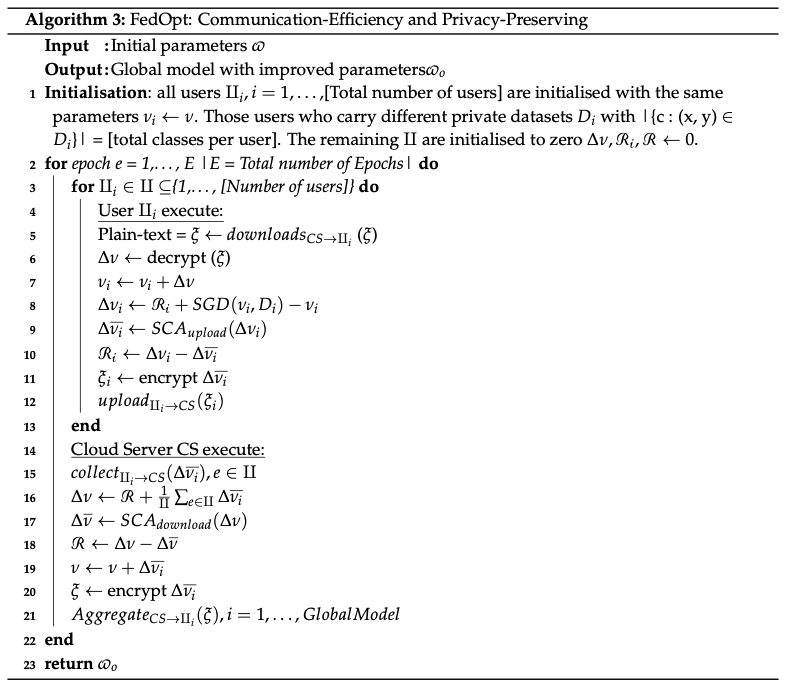
\includegraphics[width=0.8\textwidth]{src/img/Algorithm3.png}
        \end{figure}

    
    \end{frame}

    \begin{frame}
        \frametitle{
            \href{https://www.mdpi.com/2076-3417/10/8/2864}{
            FedOpt: Towards Communication Efficiency and
            Privacy Preservation in Federated Learning
            }
        }
        

        \begin{figure}[H]
            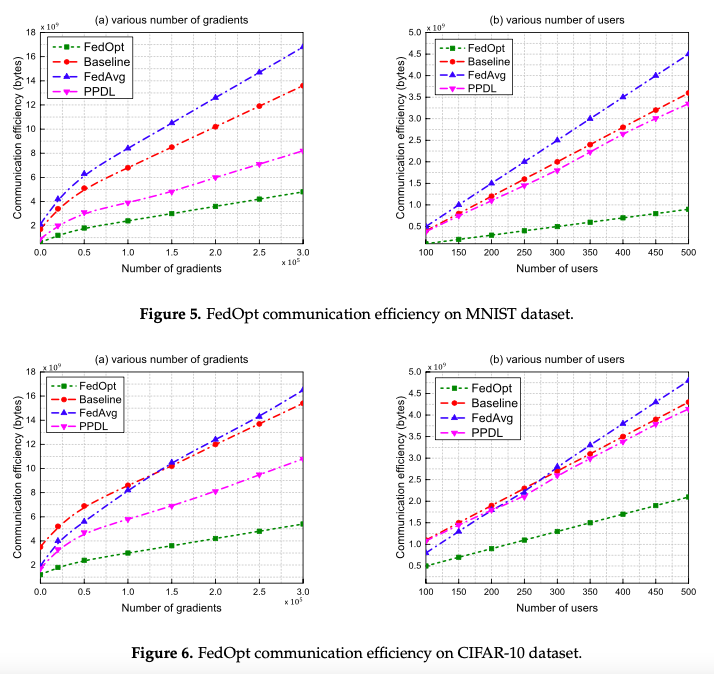
\includegraphics[width=0.8\textwidth]{src/img/Communication_Eff.png}
        \end{figure}

    
    \end{frame}

    \begin{frame}
        \frametitle{
            \href{https://www.mdpi.com/2076-3417/10/8/2864}{
            FedOpt: Towards Communication Efficiency and
            Privacy Preservation in Federated Learning
            }
        }
        

        \begin{figure}[H]
            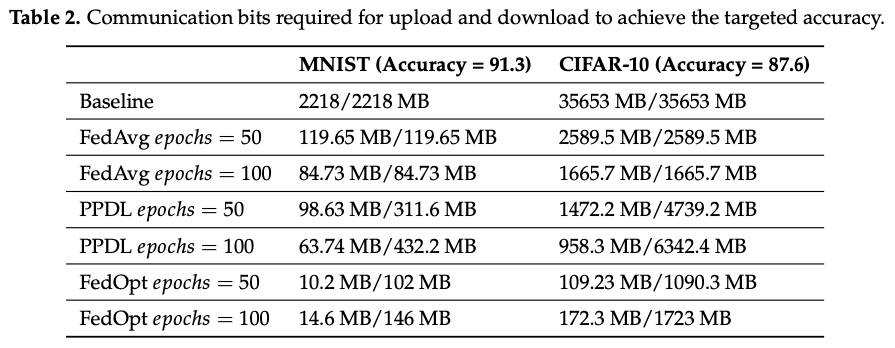
\includegraphics[width=\textwidth]{src/img/Accuracy.png}
        \end{figure}

    
    \end{frame}


    \section*{One-Shot Federated Learning}
    \begin{frame}
        \frametitle{
            \href{https://arxiv.org/pdf/1902.11175.pdf}{
                One-Shot Federated Learning
            }
        }
        
        \framesubtitle{
            Background
        }

        \textit{"In this work, we instead focus on techniques for \texttt{one-shot federated learning}, in which we learn a global model from data in the network using only a single round of communication between the devices and the central server. "}

        \textit{"Our key insight is that if each local device trains a local model to completion (as opposed to computing incremental updates as in traditional federated learning methods), we can effectively apply ensemble methods to capture global information across the device-specific models."}
        

    \end{frame}

    \begin{frame}
        \frametitle{
            \href{https://arxiv.org/pdf/1902.11175.pdf}{
                One-Shot Federated Learning
            }
        }
        
        \framesubtitle{
            Methods
        }

        \textbf{Local}: for $ m $ devices, each device $ t \in [m] $ possesses local data $ X_t \in \mathcal{R}^{d \times n_t} $ and solves:
        $$
            \min_{w_t \in \mathcal{R}^d}\lbrace{ \mathcal{P}{w_t} := \frac{1}{n_t} \sum_{i=1}^{n_t} \ell_i(x_i^T + w_t) + \frac{\lambda}{2} \left\|w_t\right\|^2 }\rbrace
        $$
        where the vector $ \{x_i\}^{n_t}_{i=1} \in X_t $ and $ \ell_i $ 
        are real-valued convex loss functions (i.e. hinge loss). In the kernelized setting, we solve the dual formulation of this problem:
        $$
            \max_{\alpha_t \in \mathcal{R}^{n_t}} 
            \lbrace{
                -\frac{1}{2\lambda n^2_t} 
                \alpha^T_t \phi (X_t)^T \phi (X_t) 
                \alpha_t + \frac{1}{n_t} 
                \sum^{n_t}_{i=1} - \ell^* (-[\alpha_t]_i)
            }\rbrace
        $$
        where $ \phi (X_t)^T \phi (X_t) $ can be replaced with $ k(X_t, X_t) $ using kernel trick.
    \end{frame} 
    
    \begin{frame}
        \frametitle{
            \href{https://arxiv.org/pdf/1902.11175.pdf}{
                One-Shot Federated Learning
            }
        }
        
        \framesubtitle{
            Methods
        }

        \textbf{Ensemble}: 
        \begin{enumerate}
            \item Cross-Validation (CV) Selection: Devices only share their local models if they achieve some baseline performance (e.g., in terms of ROC AUC) on their local validation data, with the baselines determined in advance by the server. The server ensembles the k best performing models from this subset of local models.
            \item Data Selection: Devices only share their local models if they have some baseline amount of local training data, with the baseline determined in advance by the server. The server ensembles models from these local models trained on the top k largest data sets.
            \item Random Selection: The server randomly selects k devices from the network and creates an ensemble from the corresponding local models.
        \end{enumerate}
        The final ensemble $ F_k $ of $ k $ device models is constructed by averaging the predictions of each model.
        

    \end{frame}

    \begin{frame}
        \frametitle{
            \href{https://arxiv.org/pdf/1902.11175.pdf}{
                One-Shot Federated Learning
            }
        }
        
        \framesubtitle{
            Methods
        }

        \textbf{Distillation (Semi-Supervised)}: 

        When the amount of clients is large... 

        When the central server has access to unlabelled public proxy data, $ F_k $ can be compressed into a smaller model, $ f^{\prime} $, via distillation.

        \texttt{New Method}: For proxy data $ x^{\prime}_1, ..., x^{\prime}_l$, we generate corresponding "soft" labels $ F_k(x^{\prime}) $, ...,. In particular, we perform distillation in the dual by minimizing the L2 difference in predictions between the student and teacher on the proxy data:
        $$
            \min_{\alpha^\prime \in \mathcal{R}^l} \frac{1}{l} \sum^l_{i=1}(F(x^\prime_i) - \sum_{j=1}^l \alpha^\prime_j k(x_j^\prime, x_i^\prime))^2
        $$
        to produce a distilled model $ f^\prime(x) = \sum^l_i=1 \alpha_i \phi (x^\prime_i) $. When there are privacy concerns with sharing local models between devices (e.g., for dual SVMs, which require local support vectors to be shared), distillation not only helps to compress the model but also enables privacy-preservin learning.
        

    \end{frame}


    \begin{frame}
        \frametitle{
            \href{https://arxiv.org/pdf/1902.11175.pdf}{
                One-Shot Federated Learning
            }
        }
        
        \framesubtitle{
            Result
        }

        \begin{figure}
            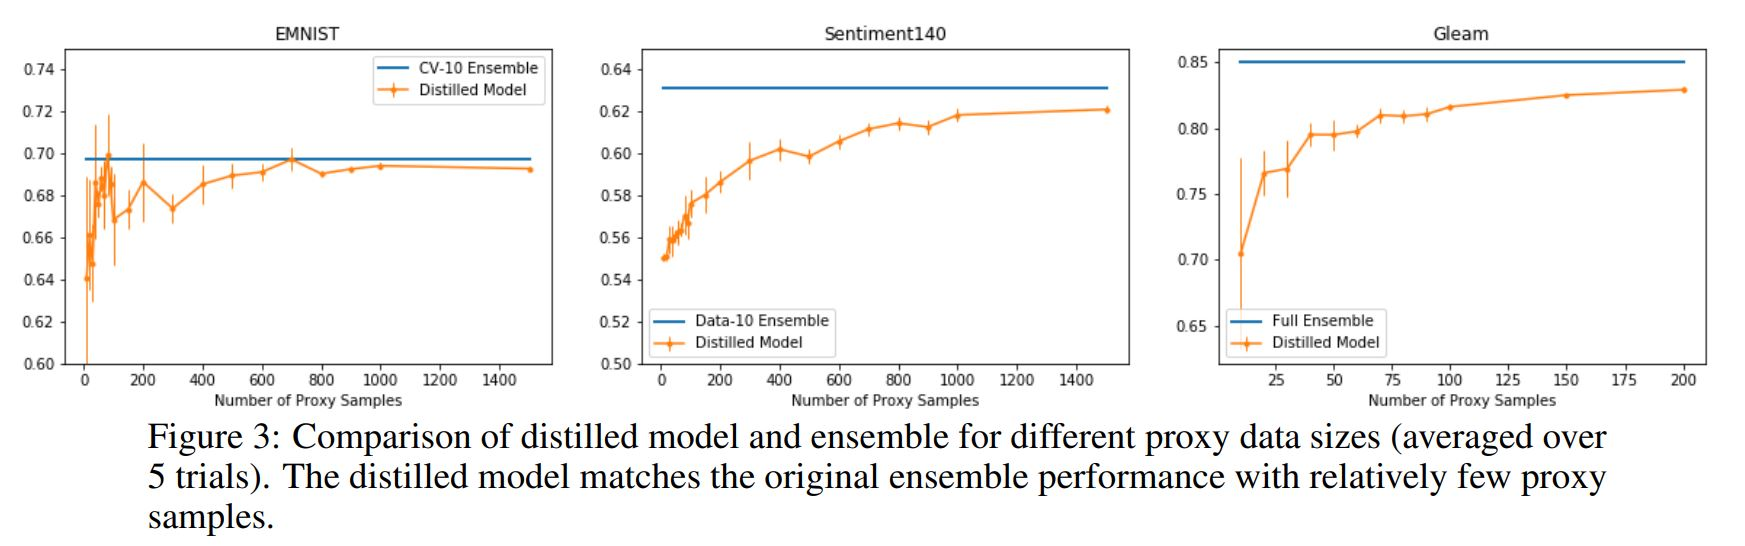
\includegraphics[width=\textwidth]{src/img/OneShotFedResult.JPG}
        \end{figure}
        {\small
            \begin{itemize}
                \item[EMNIST]{ 
                    Handwritten characters authored by different individuals (devices). We predict between lowercase and uppercase letters
                }
                \item[Sentiment140]{
                    Binary sentiment detection on tweets from different users (devices). We use a bag-of-words representation to featurize tweets
                } 
                \item[Gleam]{
                    Two hours of high resolution Google Glass sensor data corresponding to different activities. We predict between eating and other activities (walking, talking, etc)
                }
            \end{itemize}
        }

    \end{frame}

    \section*{Expanding the reach of federated learning by reducing client resource requirement}

    \begin{frame}
        \frametitle{
            \href{https://arxiv.org/pdf/1812.07210.pdf}{
            Expanding the reach of federated learning by reducing client resource requirement
            }
        }

        \framesubtitle{
            Overview 
        }

        \begin{figure}
            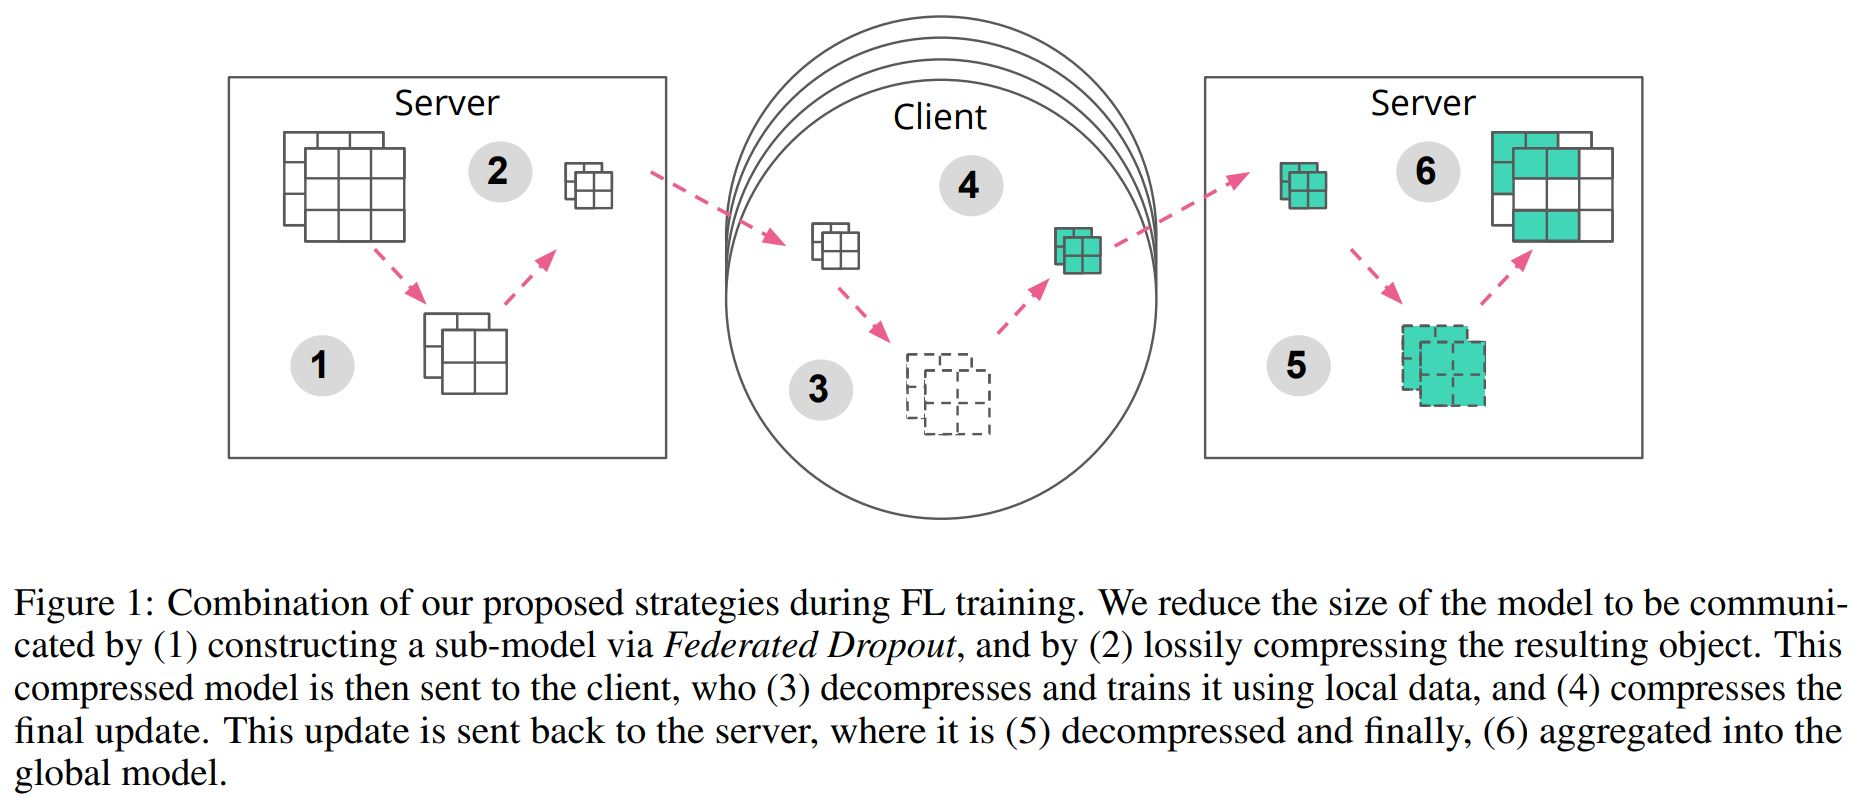
\includegraphics[width=\textwidth]{src/img/RCRRStructure.JPG}
        \end{figure}


    \end{frame}

    \begin{frame}
        \frametitle{
            \href{https://arxiv.org/pdf/1812.07210.pdf}{
            Expanding the reach of federated learning by reducing client resource requirement
            }
        }

        \framesubtitle{
            Method1: Lossy Compression 
        }

        We reshape each to-be-compressed weight matrix in our model into a vector w and (1) apply a \textit{basis transform} to it. We then (2) \textit{subsample} and (3) \textit{quantize} the resulting vector and finally send it through the network. Once received, we simply execute the respective inverse transformations to finally obtain a noisy version of $ \textbf{w} $.


    \end{frame}

    \begin{frame}
        \frametitle{
            \href{https://arxiv.org/pdf/1812.07210.pdf}{
            Expanding the reach of federated learning by reducing client resource requirement
            }
        }

        \framesubtitle{
            Method2: Federated Dropout 
        }

        \begin{figure}
            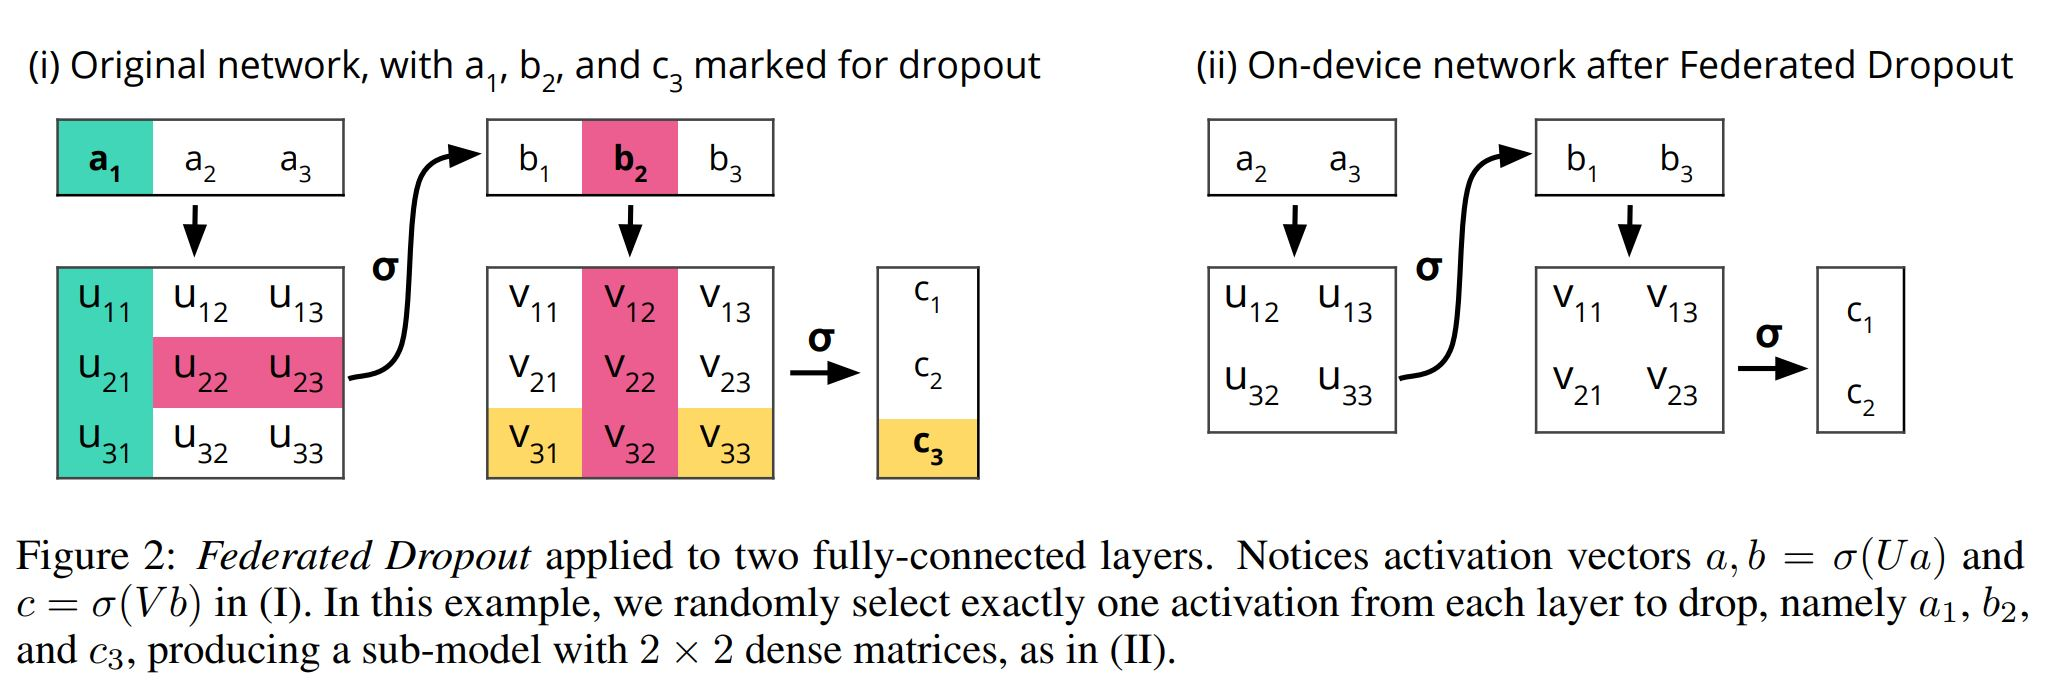
\includegraphics[width=\textwidth]{src/img/FedDropout.JPG}
        \end{figure}
    \end{frame}

    \begin{frame}
        
        \frametitle{
            \href{https://arxiv.org/pdf/1812.07210.pdf}{
            Expanding the reach of federated learning by reducing client resource requirement
            }
        }

        \framesubtitle{
            Method2: Federated Dropout 
        }


        Traditional dropout: hidden units are multiplied by a random binary mask in order to drop an expected fraction of neurons during each training pass through the network. Because the mask changes in each pass, each pass is effectively computing a gradient with respect to a different sub-model. These sub-models can have different sizes (architectures) depending on how many neurons are dropped in each layer. Now, even though some units are dropped, in all implementations we are aware of, activations are still multiplied with the original weight matrices, they just have
        some useless rows and columns.

    \end{frame}

    \begin{frame}
        
        \frametitle{
            \href{https://arxiv.org/pdf/1812.07210.pdf}{
            Expanding the reach of federated learning by reducing client resource requirement
            }
        }

        \framesubtitle{
            Method2: Federated Dropout 
        }


        To extend this idea to FL and realize communication and computation savings, we instead zero out a fixed number of
        activations at each fully-connected layer, so all possible sub-models have the same reduced architecture; see Figure 2.
        The server can map the necessary values into this reduced architecture, meaning only the necessary coefficients are
        transmitted to the client, re-packed as smaller dense matrices. The client (which may be fully unaware of the original
        model’s architecture) trains its sub-model and sends its update, which the server then maps back to the global model2
        . For convolutional layers, zeroing out activations would not realize any space savings, so we instead drop out a fixed
        percentage of filters.

    \end{frame}


    \begin{frame}
        
        \frametitle{
            \href{https://arxiv.org/pdf/1812.07210.pdf}{
            Expanding the reach of federated learning by reducing client resource requirement
            }
        }

        \framesubtitle{
            Method2: Federated Dropout 
        }

        This technique brings two additional benefits beyond savings in server-to-client communication. First, the size of the
        client-to-server updates is also reduced. Second, the local training procedure now requires a smaller number of FLOPS
        per gradient evaluation, either because all matrix-multiplies are now of smaller dimensions (for fully-connected layers)
        or because less filters have to be applied (for convolutional ones). Thus, we reduce local computational costs.

    \end{frame}


    
    \begin{frame}
        
        \frametitle{
            \href{https://arxiv.org/pdf/1812.07210.pdf}{
            Expanding the reach of federated learning by reducing client resource requirement
            }
        }

        \framesubtitle{
            Results
        }


        \begin{figure}
            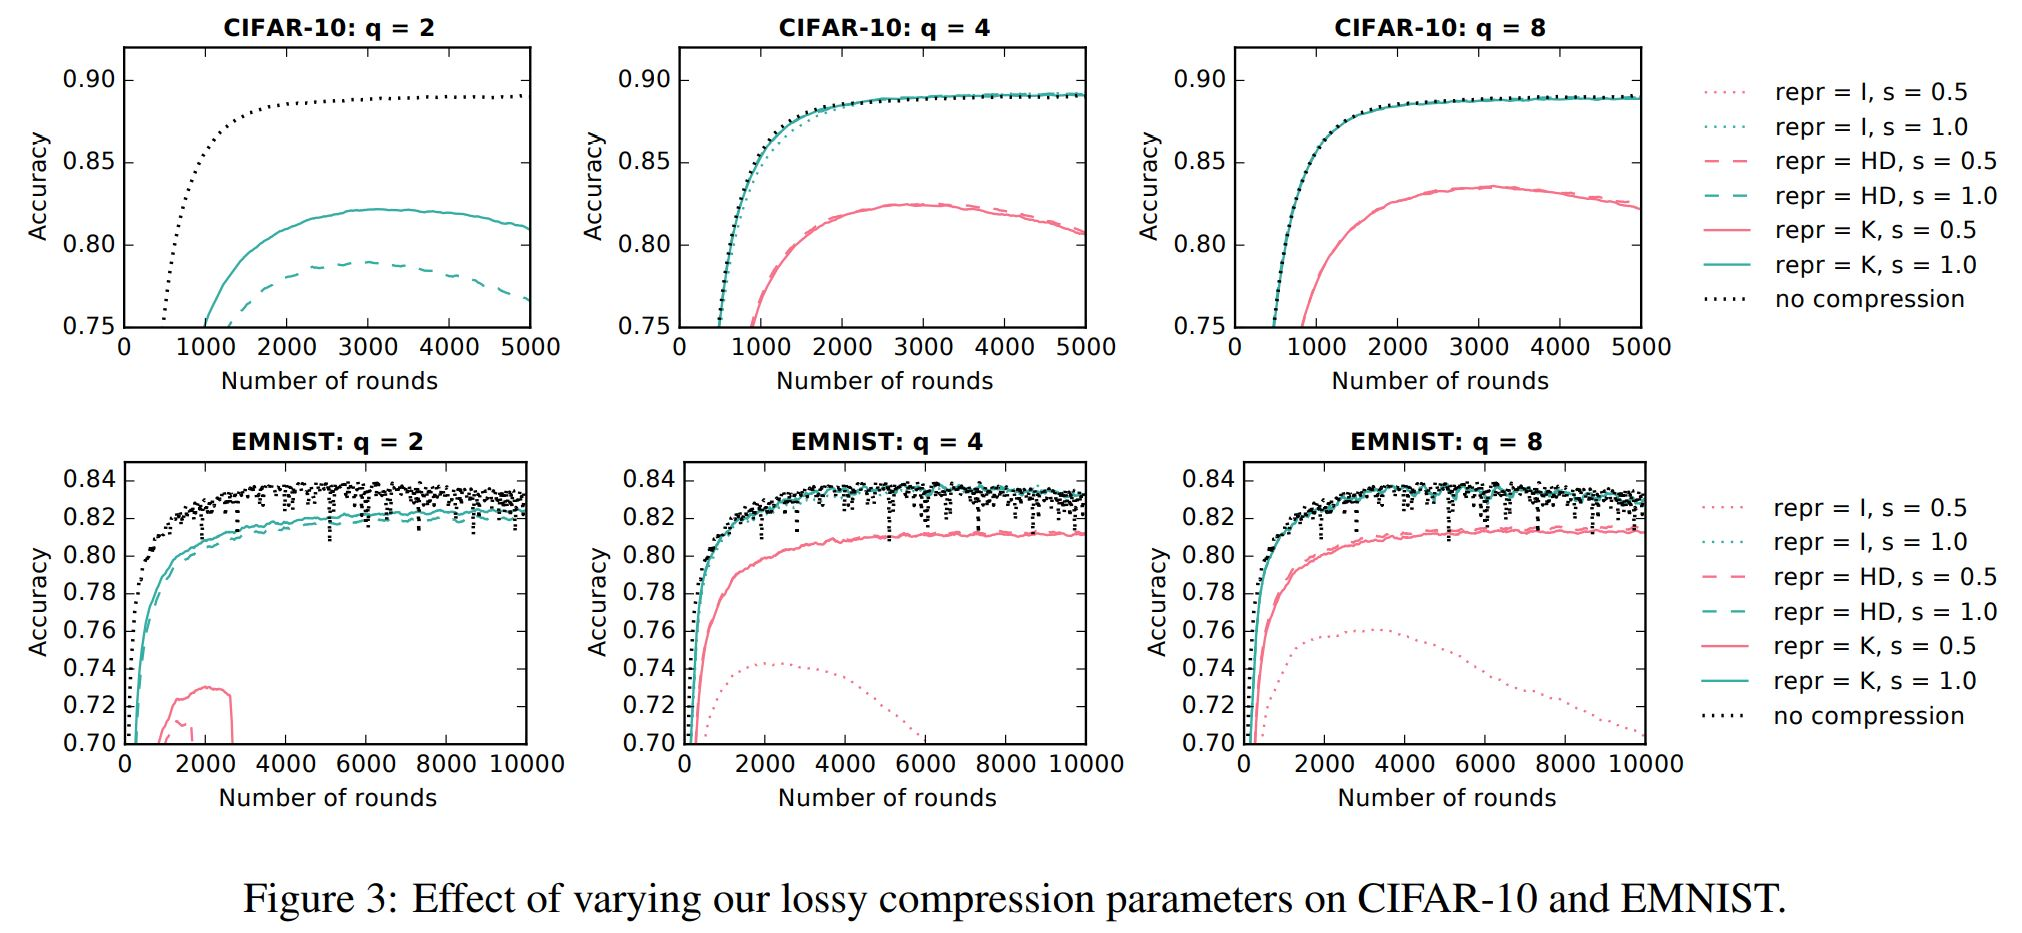
\includegraphics[width=\textwidth]{src/img/DpR1.JPG}
        \end{figure}

    \end{frame}

    \begin{frame}
        
        \frametitle{
            \href{https://arxiv.org/pdf/1812.07210.pdf}{
            Expanding the reach of federated learning by reducing client resource requirement
            }
        }

        \framesubtitle{
            Results
        }


        \begin{figure}
            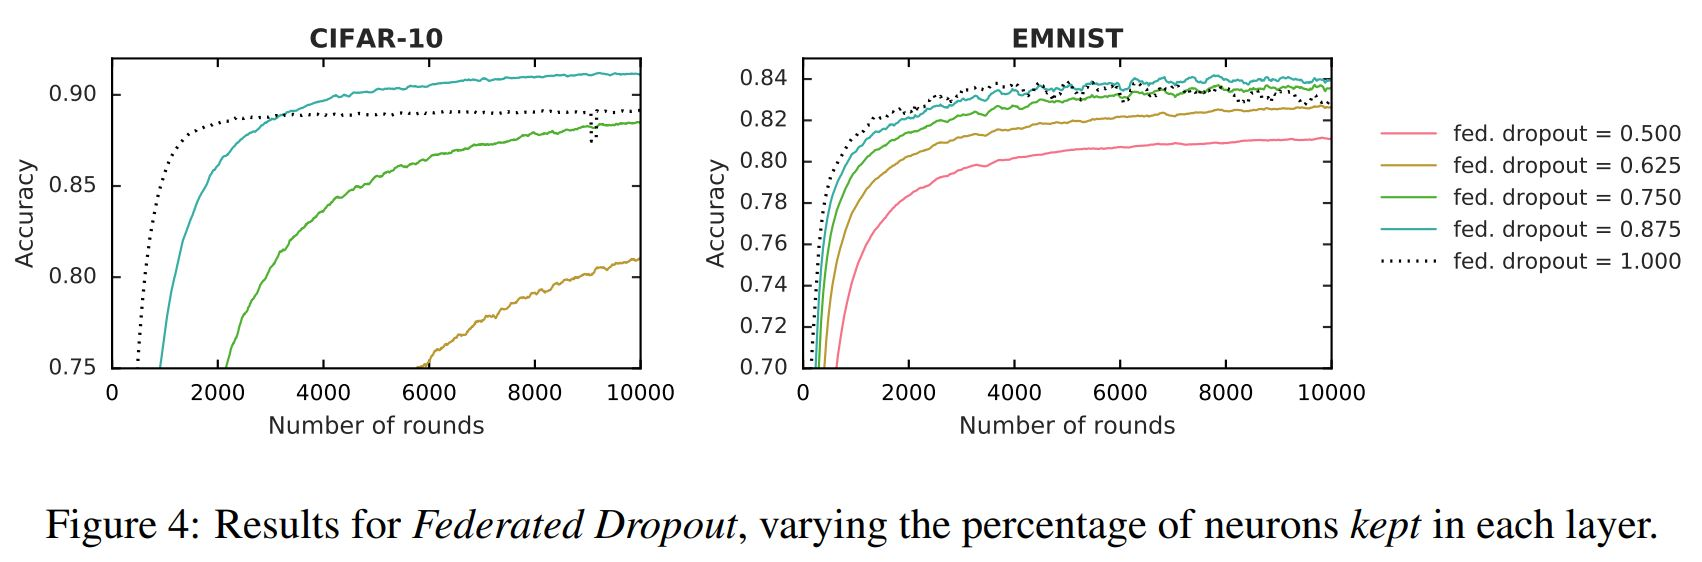
\includegraphics[width=\textwidth]{src/img/DpR2.JPG}
        \end{figure}

    \end{frame}

    % Reference 
    \begin{frame}
        \frametitle{
            Reference
        }
        
        % Reference below
        % \bibliography{src/citations/ref.bib}
        \nocite{*}
        \bibliography{src/citations/ref.bib}

    \end{frame}

\end{document}